
\documentclass[12pt,AutoFakeBold]{article} 

\usepackage[智能数据挖掘]{XDUreport}  % 科目名称
\problem{PAM 算法练习}  % 请在此处填写问题内容
% 其他参数在宏包中进行更改,其中学院,班级,姓名,学号均在sty宏包内进行更改
% \usepackage{fourier}  % 这是 fourier 字体,更柔和 

%% 如果你需要中文的一级标题编号,如“一、”、“二、”等,请把下面两行取消注释
% \RequirePackage{zhnumber} % change section number to chinese
% \titleformat{\section}{\Large\bfseries\rmfamily}{\zhnum{section}、}{0em}{}
%\usepackage[table,xcdraw]{xcolor}
%\definecolor{lightblue}{RGB}{222, 234, 246}

% 文档开始
        
\begin{document}

\maketitle
\setcounter{tocdepth}{2}

\tableofcontents  % 生成目录

% 正文标题
\makeatletter
\begin{center}
    \LARGE \textbf{\textsf{\@problem}}
\end{center}
\makeatother

% 正文开始

\section{问题描述}

编程实现 PAM 对部分 waveform 数据集加 20\% 的高斯噪声;同时对一副噪声图像进行分割; 

\section{原理分析}

\subsection{waveform 数据集}

waveform 数据集是订货书的波形域,共有 5000 个样本,3 种标签,21 个属性,每个属性是 0 到 6 之间的连续值,没有缺失属性值,每个类别占 33\%,近邻算法准确率在 78\% 左右。本题中我对 20 \% 的数据添加了高斯噪声。


\subsection{PAM 算法}

PAM (Partition Around Medoids) 方法于1987年提出,用于l1范数和其他距离的工作。k-medoid 是一种经典的聚类分割技术,它将 n 个对象的数据集聚为 k 个聚类,假设聚类的数量 k 是先验的。如果未知,则可以使用诸如轮廓的方法来确定 k。PAM 利用了贪婪搜索,不一定可以找到最优解,但是比穷尽搜索更快。

对比 k-means,它对噪声和异常值更具鲁棒性。k-means 是每次选簇的均值作为新的中心,迭代直到簇中对象分布不再变化。其缺点是对于离群点是敏感的,因为一个具有很大极端值的对象会扭曲数据分布。那么我们可以考虑新的簇中心不选择均值而是选择簇内的某个对象,只要使总的代价降低就可以。k-medoids 算法比 k-menas 对于噪声和孤立点更鲁棒,因为它最小化相异点对的和 (minimizes a sum of pairwise dissimilarities) 而不是欧式距离的平方和 (sum of squared Euclidean distances)。一个中心点 (medoid) 可以这么定义:簇中某点的平均差异性在这一簇中所有点中最小。

\subsection{图像分割}

在计算机视觉领域,图像分割(segmentation)指的是将数字图像细分为多个图像子区域(像素的集合)(也被称作超像素)的过程。图像分割的目的是简化或改变图像的表示形式,使得图像更容易理解和分析。图像分割通常用于定位图像中的物体和边界(线,曲线等)。更精确的,图像分割是对图像中的每个像素加标签的一个过程,这一过程使得具有相同标签的像素具有某种共同视觉特性。

\section{实验过程}

\subsection{waveform 数据集聚类}

导入数据集后发现 0 类 1657 个,1 类 1647 个,2 类1696 个,对 20\% 数据添加均值为 0,标准差为 1 的高斯噪声。然后实现 PAM 方法步骤如下:

\begin{enumerate}
\renewcommand{\labelenumi}{\bfseries \textit{Step} \theenumi.}

\item 任意选择 $k$ 个对象作为初始的簇中心点。

\item 将其余对象划分到距 $k$ 个初始类别中心最近的簇。

\item 计算所有对象与其簇中中心点的距离值,将其全部累加得到损失值,记为 cost0。

\item 随机选择一个非中心对象别临时试替换 $k$ 个簇中心对象中的一个,重新分簇,计算得到一个损失值 cost。

\item 如果这个损失值 cost 小于 \textbf{\textit{Step} 3} 中得到的 cost0,则将这个最小损失值计算时对应的非中心点和中心点交换,更新 cost0。

\item 重复 \textbf{\textit{Step} 4$\sim$6} 步骤,重复迭代直至收敛。
\end{enumerate}

设置迭代次数为 10,聚类中心和聚类划分结果见附录,选取第 7 维和第 10 维的数据进行可视化展示,如图 \ref{fig:plot1} 所示。

\begin{figure}[htbp]
	\centering
    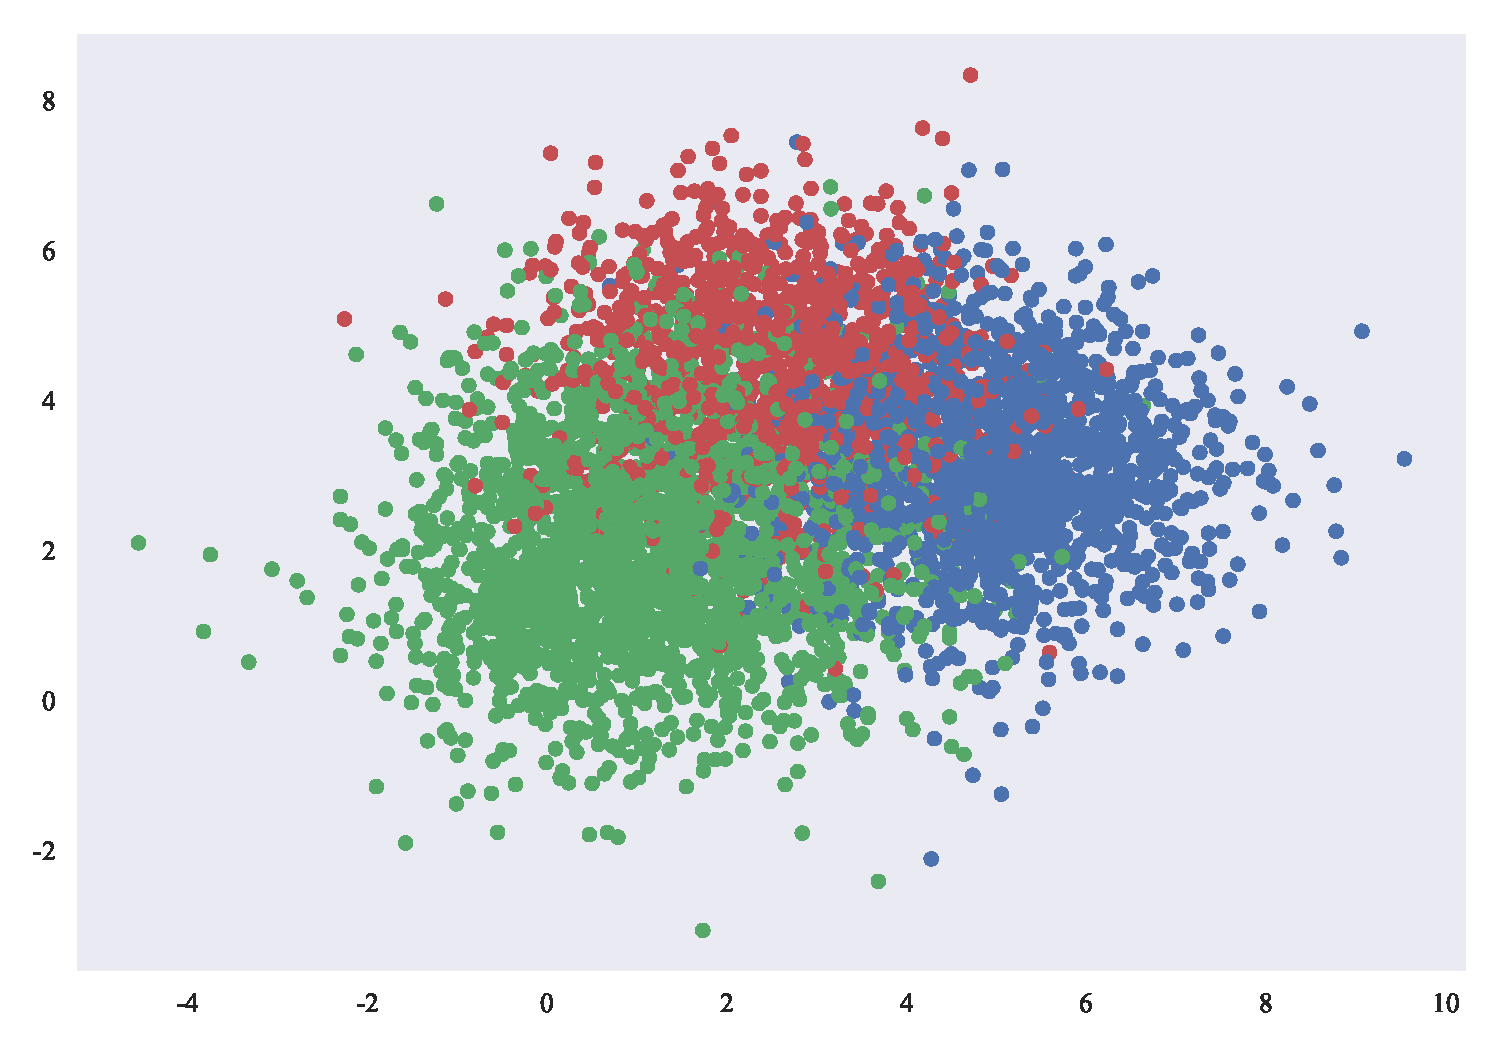
\includegraphics[width=0.7\textwidth]{plot1.pdf}
    \caption{PAM 算法聚类后第 7 维和第 10 维可视化展示} \label{fig:plot1}
\end{figure}

\subsection{噪声图像分割}

使用 Python 库函数 \lstinline[language=Python]|random.gauss(mu, sigma)| 对如图 \ref{fig:original image} 所示无噪声图像每个像素点添加均值为 0 标准差为 50 的噪声,得到如图 \ref{fig:noise image} 所示的噪声图像。

\begin{figure}[htbp]
	\centering
	\begin{minipage}[t]{0.48\textwidth}
		\centering
		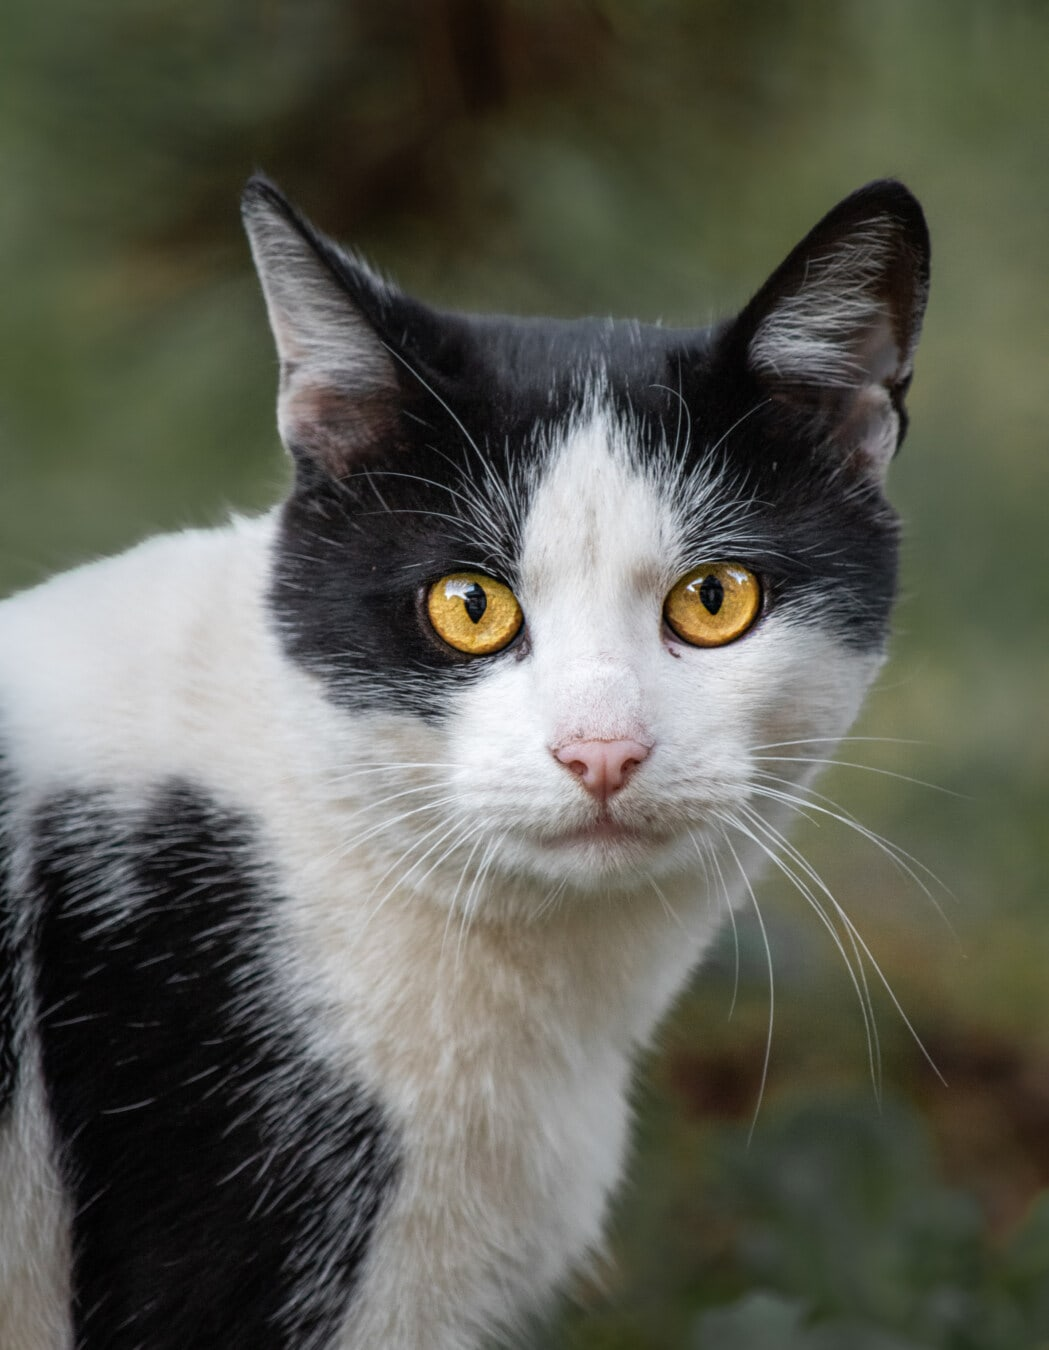
\includegraphics[width=7cm]{image-1080x1350.jpg}
		\caption{原始图像} \label{fig:original image}
	\end{minipage}
	\begin{minipage}[t]{0.48\textwidth}
		\centering
		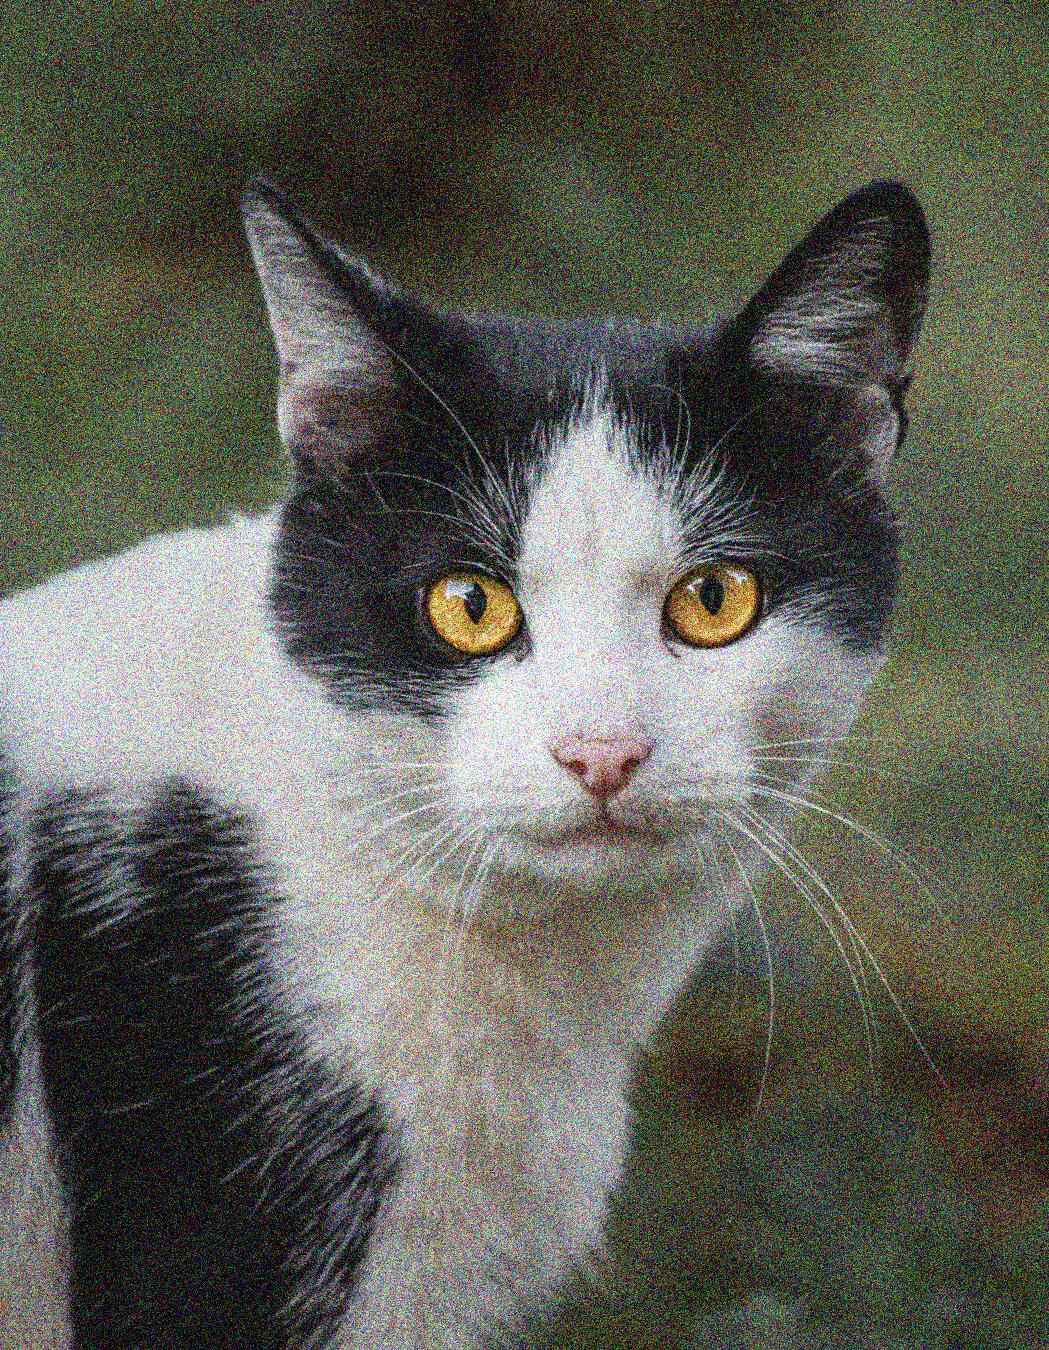
\includegraphics[width=7cm]{noise_image.jpg}
		\caption{20\% 数据添加高斯噪声后的噪声图像} \label{fig:noise image}
	\end{minipage}
\end{figure}


首先尝试使用 k-means 对噪声图像进行分割,分别取 $k=4$ 和 $k=8$ 得到如图 \ref{fig:cluster4} 和图 \ref{fig:cluster8} 所示的分割结果。

\begin{figure}[htbp]
	\centering
	\begin{minipage}[t]{0.48\textwidth}
		\centering
		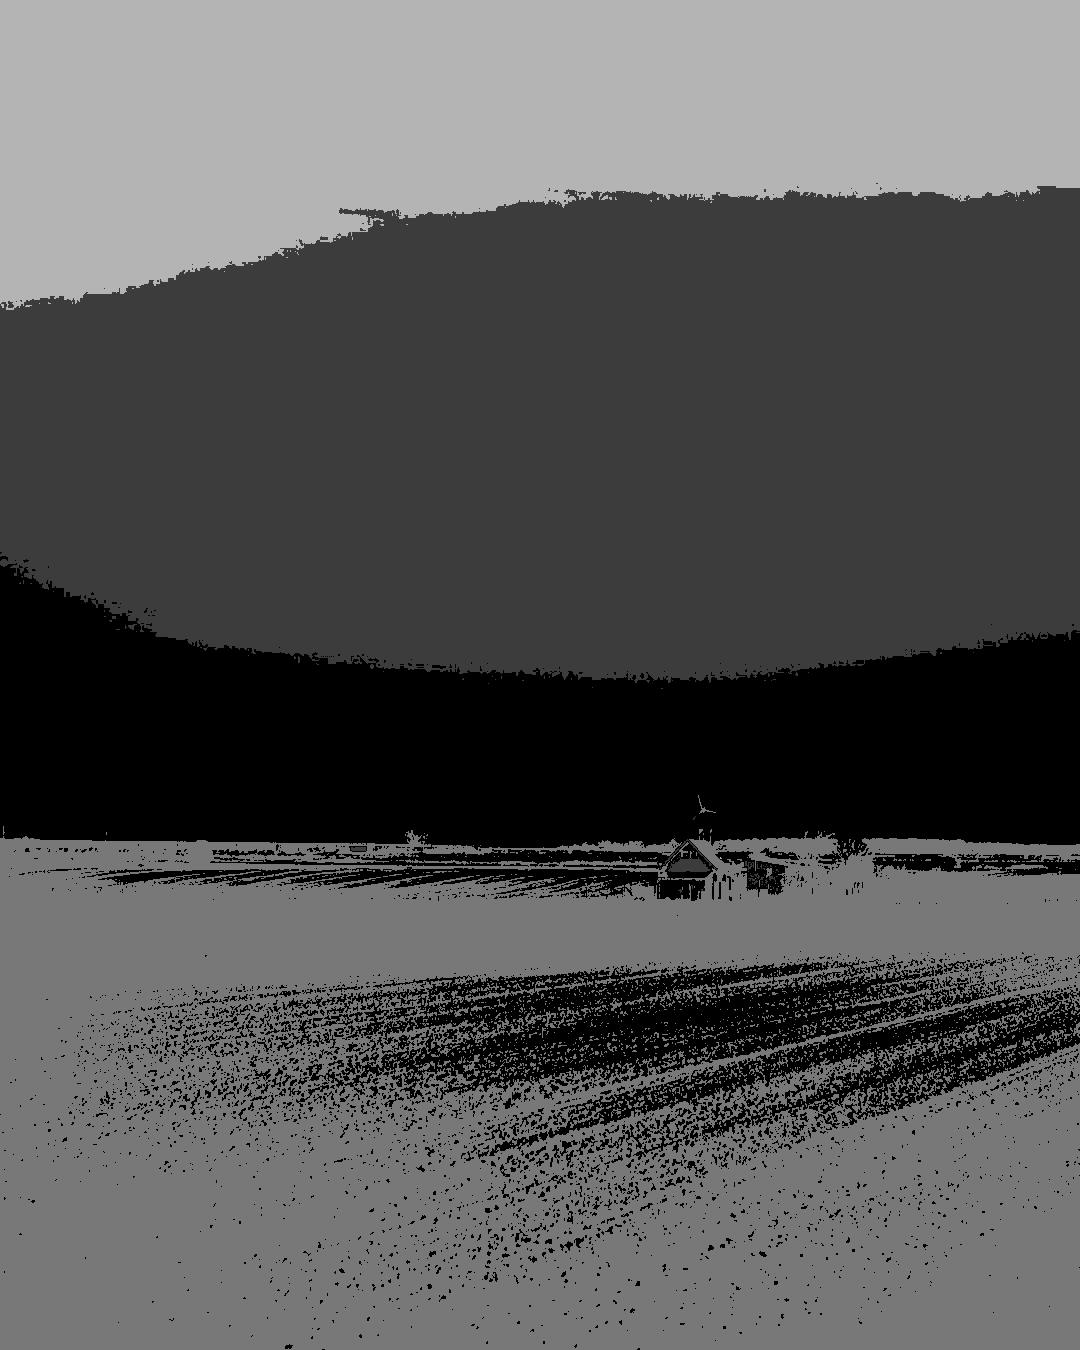
\includegraphics[width=7cm]{cluster4.jpg}
		\caption{k-means 噪声图像聚类分割 $k=4$ 时结果} \label{fig:cluster4}
	\end{minipage}
	\begin{minipage}[t]{0.48\textwidth}
		\centering
		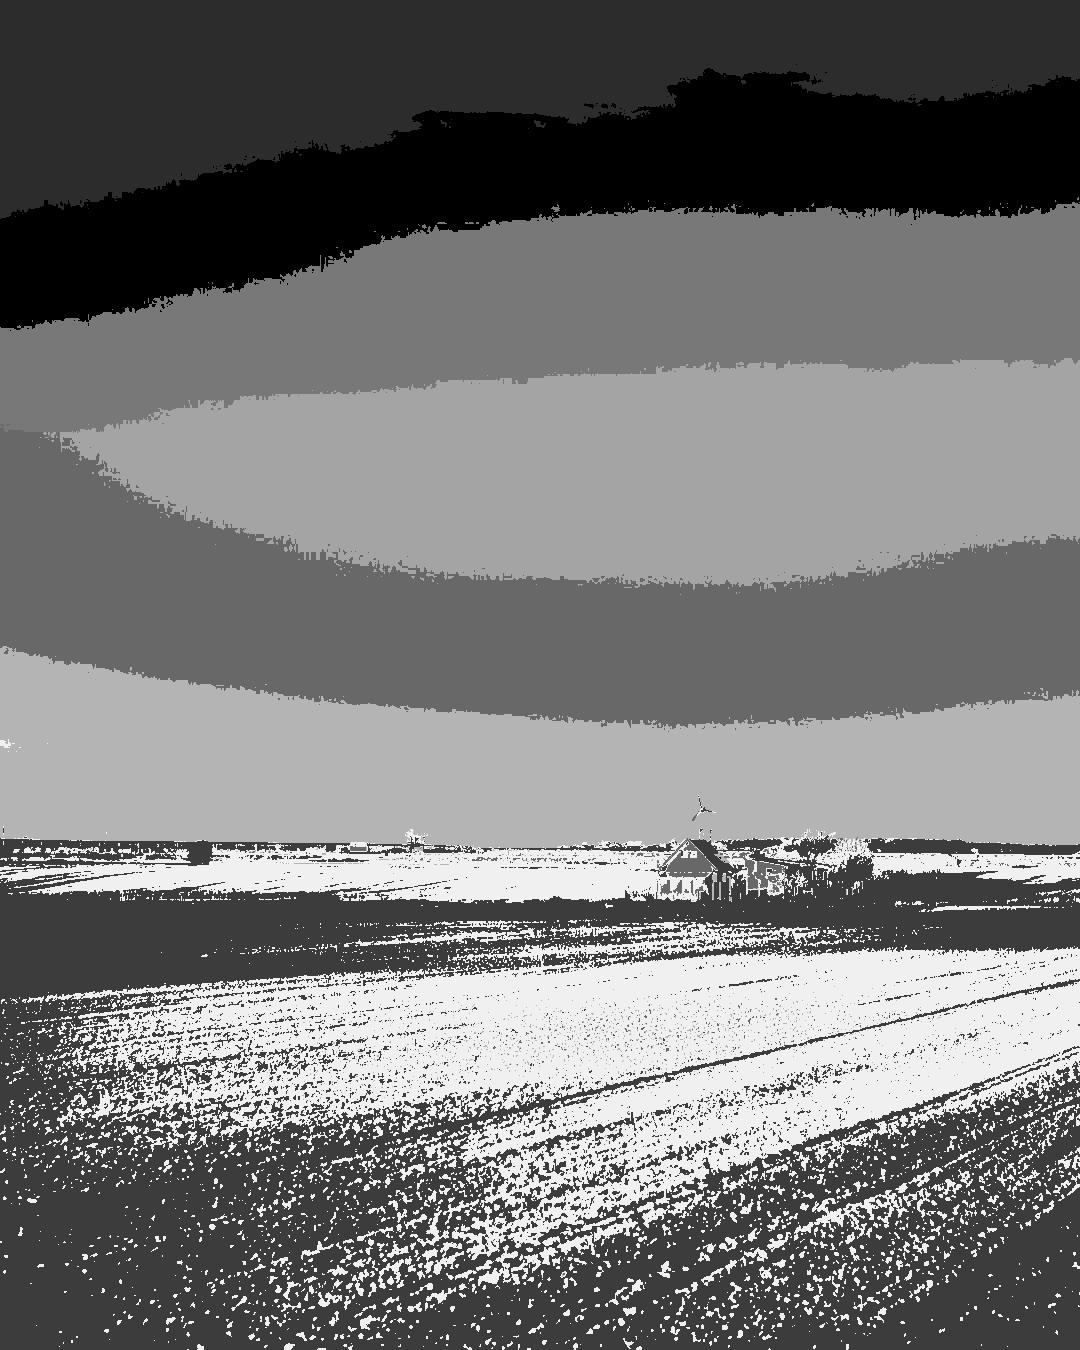
\includegraphics[width=7cm]{cluster8.jpg}
		\caption{k-means 噪声图像聚类分割 $k=8$ 时结果} \label{fig:cluster8}
	\end{minipage}
\end{figure}

然后我们用编写 PAM 算法对噪声图像进行分割,迭代次数为 5,类数分别为 3 和 6,得到分别如图 \ref{fig:output1} 和图 \ref{fig:output2} 所示的结果。

\begin{figure}[htbp]
	\centering
    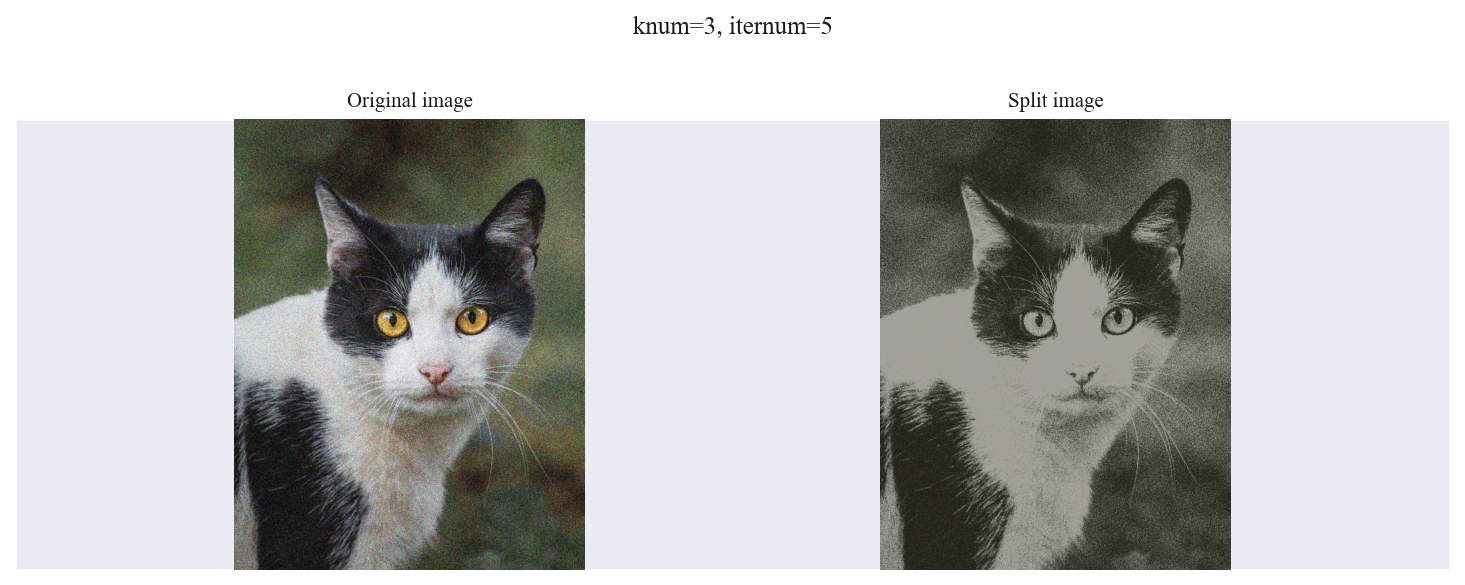
\includegraphics[width=\textwidth]{output1.png}
    \caption{PAM 算法对噪声图像进行分割类别数为 3 时结果} \label{fig:output1}
\end{figure}

\begin{figure}[htbp]
	\centering
    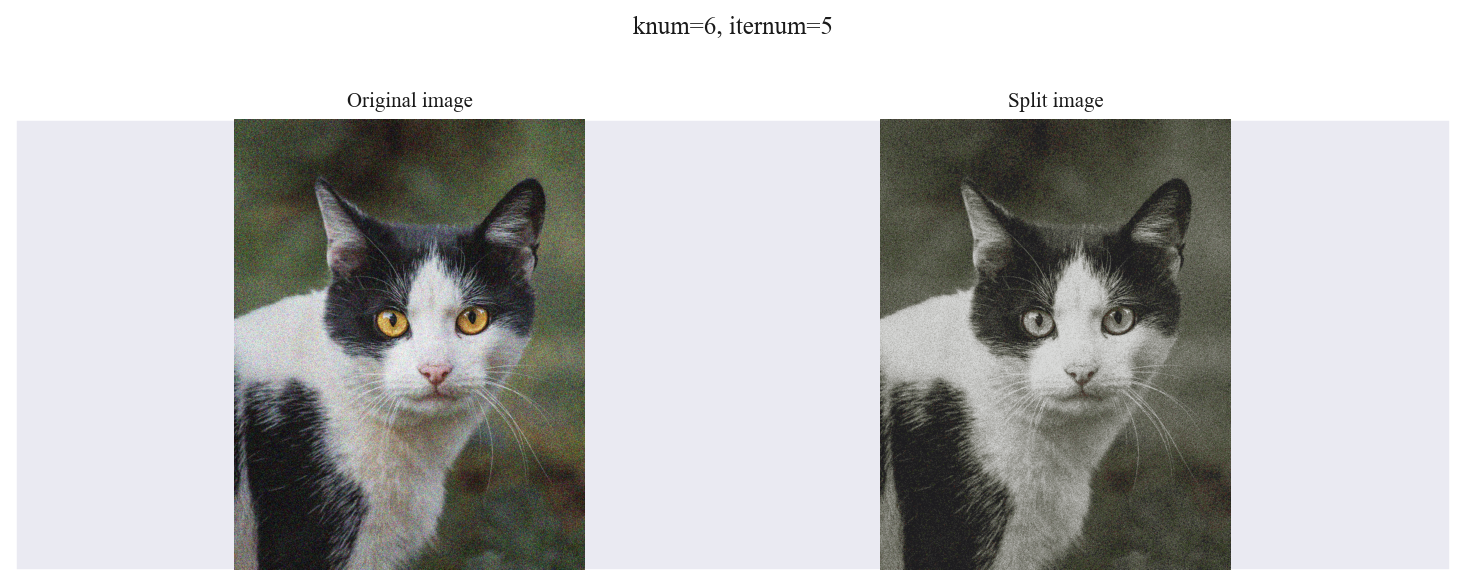
\includegraphics[width=\textwidth]{output2.png}
    \caption{PAM 算法对噪声图像进行分割类别数为 6 时结果} \label{fig:output2}
\end{figure}

可以得出结论,PAM 算法相比于 k-means 算法,具有更好的鲁棒性。在一定迭代次数下,设置类别数越多,图像分割越明显,细节越丰富。但迭代次数的增加并不会导致图像分割效果变好,并且程序的运行时间会随着类别数、最大迭代次数的增加而增加。

\newpage

\includepdfset{pagecommand={\thispagestyle{fancy}}} 
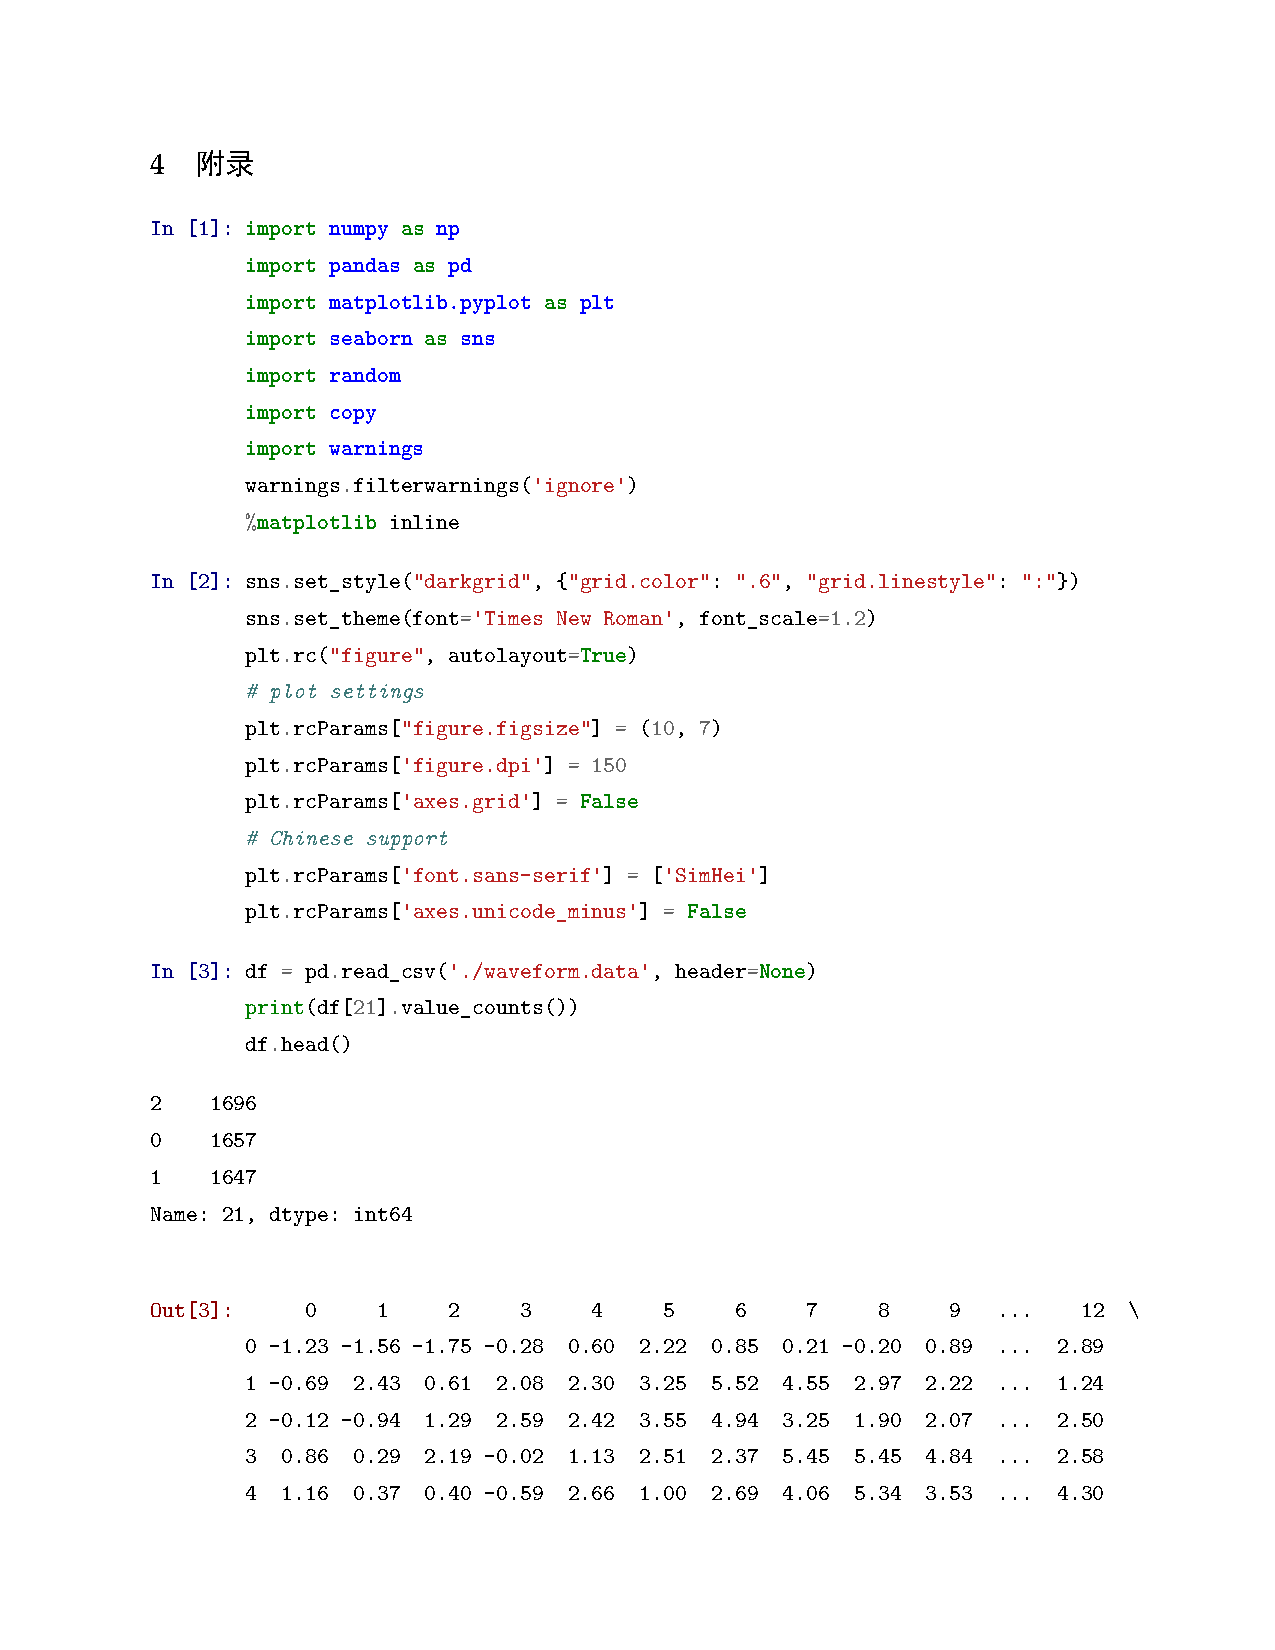
\includepdf[addtotoc={1,section,1,附录,appendix}, pages={1-11}]{PAM.pdf}

% % 参考文献,此处以 MLA 引用格式为例

% \begin{thebibliography}{9}
%     \bibitem{1} Clemente, Filipe Manuel, et al. "General network analysis of national soccer teams in FIFA World Cup 2014." \emph{International Journal of Performance Analysis in Sport} 15.1 (2015): 80-96.
%     \bibitem{3} Dijkstra, Edsger Wybe. "A Note on Two Problems in Connexion With Graphs." \emph{Numerische Mathematik} 1(1959):269-271.
%     \bibitem{4} Ahnert, Sebastian E., et al. "Ensemble approach to the analysis of weighted networks.." \emph{Physical Review E} 76.1 (2007).
%     \bibitem{5} Wong, J. A. Hartiganm. A. . "Algorithm AS 136: A K-Means Clustering Algorithm." \emph{Journal of the Royal Statistical Society. Series C (Applied Statistics)} 28.1(1979):100-108.
%     \bibitem{6} Buldu, J. M., et al. "Defining a historic football team: Using Network Science to analyze Guardiola’s F.C. Barcelona." \emph{Scientific Reports} 9.1 (2019): 1-14.
%     \bibitem{7} \emph{Balotelli sends Italy past Germany}. (2012). Retrieved December 10, 2014, from\url{https://www.uefa.com/uefaeuro/season=2012/matches/round=15174/match=2003379/index.html}
%     \bibitem{8} Sigari, Mohamad Hoseyn, et al. "Counterattack detection in broadcast soccer videos using camera motion estimation." \emph{international symposium on artificial intelligence} (2015): 101-106.
%     \bibitem{9} Abdelmahmoud Hassan Elsheikh. \emph{Effect of Leadership Intensity on Integrating Some Formal and Informal Organizational Efforts for Community Development in Khartoum Province}. 2016.
% \end{thebibliography}


% \includepdf[pages={1,2}]{Memo.pdf} 
% 可以直接导入pdf页面
% \newpage
% \begin{appendices}  % 附录环境
% \section{附录}
% \end{appendices}

\end{document}  % 结束